\chapter{Pre-integrazione}


\section{Studio frontend}
Per creare una chat nei moderni siti web dinamici \'e stato necessario lo studio di un linguaggio che sicuramente ha modernizzato lo sviluppo web cio\'e JavaScript soprattutto per la quantit\'a impressionante di framework sviluppati con questa tecnologia.
\'E un linguaggio interpretato, che ha molto poco a che fare con il quasi omonimo Java, la prima versione venne rilasciata nel 1995 con l'obbiettivo di arricchire le pagine web aggiungendo alcune forme di dinamicit\'a. L'utilizzo in una pagina \'e possibile solo se il browser del client possiede un supporto a interpretare il linguaggio, questa scelta di mantenere la responsabilit\'a a livello client \'e stata fatta per non sovracaricare troppo il server che riliasciava il servizio web relativo.
\iffalse 
<studio di angularjs nel libro (vedi https://github.com/Wabri/UniversityInternship#day-01-020518--55-ore)>
\fi
Le prime fasi di tirocinio le ho concentrate sull'apprendimento dei vari strumenti necessari per comprendere l'architettura della web application formata principalmente da codice HTML con direttive AngularJS e Javascript, tenuti insieme dal MVC (Model View Controller).
Il MVC \'e un pattern architetturale basato su 3 componenti che hanno lo scopo di usare e gestire i dati con compiti diversi: il model deve gestire i dati e fornire metodi per usarli nonch\'e la logica e le regole dell'applicazione, il view ha lo scopo di rappresentare i dati sotto forma di informazione in modo tale da interagire con l'utente che li visualizzer\'a, e infine il controller che attraverso istruzioni fornite dall'utente modifica lo stato degli altri 2 componenti modificando i dati gestiti dal controller o indicando una modalit\'a differente di visualizzazione dei dati al view.
\begin{figure}[H]
 \centering
  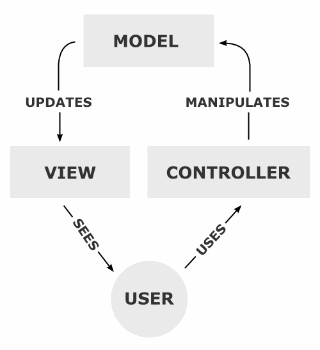
\includegraphics[width=0.3\textwidth]{img/MVC-Process.png}
 \caption{MVC}
 \end{figure}
Questa struttura viene usata principalmente per dividere la logica di business, che \'e la parte di eleborazione dati, con l'interfaccia utente, migliorando quindi l'organizzazione dei processi interni di una application. 
L'utilizzo di questo pattern direttamente sul client ha permesso un cambiamento importante per quanto riguarda le dynamic pages, cio\'e quello di non eseguire un redirect per modificare la pagina ma eseguendo chiamate asincrone al server. 
Con il tempo \'e stato necessario fornire un framework che implementasse queste logiche riducendo i tempi di sviluppo andando a generalizzare tutti quei comportamenti classici del pattern MVC, se si parla di JavaScript senza alcun dubbio il framework pi\'u usato \'e AngularJs.
Questa libreria funziona per mezzo di comandi, definiti direttive, che vengono inserite direttamente nel codice HTML che permettono di eseguire una sorta di comunicazione tra le varie parti del client. Il framework viene caricato all'interno della pagina attraverso l'import definito dal tag <script> in questo modo:
\begin{lstlisting}
<script 
 src="https://ajax.googleapis.com/ajax/libs/angularjs/1.2.19/angular.js">
</script>
\end{lstlisting}
Questo script esegue una lettura dell'intera pagina dove saranno presenti le direttive che dovr\'a eseguire che modificheranno (o no) le sezioni della pagina che vogliamo essere dinamiche.





\section{Creazione della chat stand alone}
Apprese le conoscenze base di questi strumenti ho cominciato con la stesura di una prima versione della chat testuale stand alone in JavaScript. Una chat presuppone la comunicazione tra pi\'u di 2 soggetti, nel mio caso un soggetto \'e rappresentato da l'utente della banca che usa la chat e l'altro il bot, una comunicazione di questo tipo \'e possibile implementarla usando i sockets.
I sockets sono la soluzione migliore per chat real-time con comunicazioni bidirezionali tra un client e server, questo presuppone che un client mandi un messaggio in chat e il server si prenda l'incarico di ridirezionare il messaggio al destinatario effettivo. Un socket rimane attivo in ascolto su un canale di comunicazione permettendo lo scambio in input e output di messaggi e in base al tipo di messaggio il socket eseguir\'a una azione specifica che nel caso di una chat \'e stampare o inviare un messaggio. Per fare questo ho usato una libreria JavaScript chiamata socket.io (https://socket.io) che tramite il metodo emit permette di emettere un messaggio in output:
\begin{lstlisting}
// inviare un messaggio
socket.emit('text message', text);
\end{lstlisting} 
Un pacchetto trasmesso da un socket ha bisogno di 2 parametri: una chiave necessaria a riconoscere il tipo di messaggio trasmesso e un contenuto che nel nostro caso \'e il messaggio di testo.
Una volta che il messaggio viene emesso un altro socket deve riceverlo, \'e quindi necessario che il socket del controller sia sempre in ascolto di messaggi e in base al tipo del messaggio esegua una determinata azione:
\begin{lstlisting}
// connessione e gestione del messaggio
const io = require('socket.io')(server);
io.on('connection', function (socket) {
    socket.on('text message', (text) => {
        // gestione del messaggio
    });
});
\end{lstlisting}
\iffalse
https://developer.mozilla.org/en-US/docs/Web/API/SpeechRecognition
https://developer.mozilla.org/en-US/docs/Web/API/SpeechSynthesisUtterance
\fi
Uno dei motivi principali dello sviluppo di un chatbot \'e quello di permettere all'utente di parlare direttamente al bot usando la voce. Per fare questo ho dovuto usare uno strumento che trasformasse la voce catturata dal microfono in un testo, per la precisione in una stringa da poter inviare tramite il socket al controller, un tool di questo tipo \'e definito speech recognition, in italiano riconoscimento vocale.
Ho usato una libreria sviluppata da mozilla chiamata proprio SpeechRecognition che una volta impostata la lingua ha permesso di trasformare il parlato dell'utente in una stringa utilizzabile all'interno del client.
Nel codice HTML ho inserito semplicemente un bottone che una volta attivato il microfono abilita la funzione di speech recognition, una volta che l'utente smette di parlare verr\'a restituita la stringa risultante che verr\'a inviata tramite socket.
\begin{lstlisting}
// Declaration
const SpeechRecognition = window.SpeechRecognition
const recognition = new SpeechRecognition();
// Properties
recognition.lang = 'it-IT';
recognition.interimResults = false;
// event listener click button
document.querySelector('button').addEventListener('click', () => {
    recognition.start();
});
// event listener result recognition
recognition.addEventListener('result', (e) => {
    let last = e.result.length - 1; 
    let text = e.result[last][0].transcript;
    socket.emit('chat message', text);
});
// event listener end recognition
recognition.addEventListener('speechend', () => {
  recognition.stop();
});
\end{lstlisting}
Inviato il messaggio dell'utente all'intelligenza questa genera una risposta che viene stampata nella pagina, per rendere naturale la conversazione ho deciso di dare una voce al bot introducendo il procedimento inverso dello speech to text. Per fare questo ho usato la funzione fornita da mozilla chamata SpeechSynthesisUtterance che mi ha permesso di trasformare un testo in audio dando cos\'i una voce al bot.
\begin{lstlisting}
function synthVoice(text) {
    const synth = window.speechSynthesis;
    const utterance = new SpeechSynthesisUtterance();
    utterance.text = text;
    synth.speak(utterance);
}
// event bot reply
socket.on('bot reply', function (replyText) {
    synthVoice(replyText);
});
\end{lstlisting}
L'ultima cosa da fare per la parte frontend \'e stata una web interface minimale che permettesse di testare il funzionamento del bot, quindi c'era bisogno di: un bottone che attivasse lo speech to text, una casella di testo nel caso in cui non si voglia usare il microfono e 2 zone di testo dove riportare gli ultimi messaggi scambiati.
\begin{figure}[H]
 \centering
  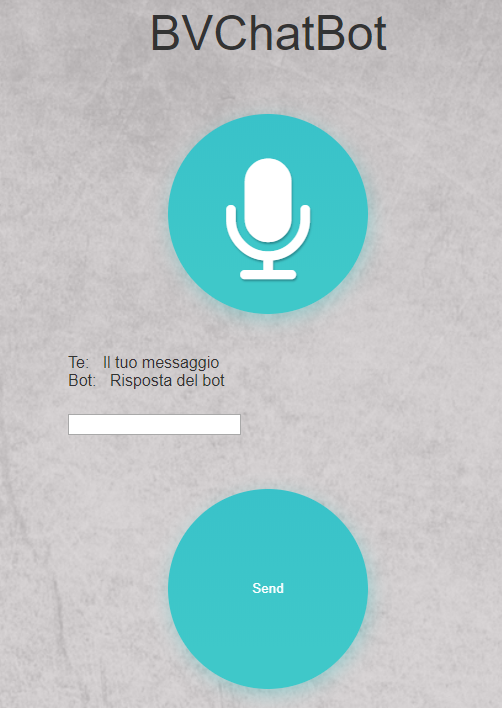
\includegraphics[width=0.4\textwidth]{img/prototype.png}
 \caption{Chat prototype}
\end{figure}
Il frontend ha avuto diverse riscritture a causa della poca esperienza in JavaScript che possedevo, l'ultima versione del prototipo \'e scritta in linguaggio TypeScript che ritengo molto pi\'u leggibile, facile da mantenere e comprendere nel lungo tempo. 
TypeScript permette di non soffrire dal passaggio da linguaggi di programmazione orientati agli oggetti a JavaScript in cui sono assenti i tipi. JavaScript \'e linguaggio tipizzato che non prevede controlli statici sui tipi di dato effettuando una conversione implicita tra i tipi, questa particolarit\'a lo rende enormemente flessibile il problema arriva quando si generano errori che difficilmente sono analizzabili a runtime. 
TypeScript \'e di per se un'estensione di JavaScript e qualsiasi script JavaScript \'e anche codice TypeScript valido. Il primo vantaggio \'e offerto dal fatto che la transizione da un progetto JavaScript esistente a TypeScript pu\'o essere fatto gradualmente, senza la necessit\'a di riscrivere tutto. Il secondo vantaggio \'e rappresentato dalla possibilit\'a di sfruttare il compilatore TypeScript su codice JavaScript standard per individuare gi\'a in fase di compilazione errori che normalmente possono sfuggire.
Avendo provato diverse architetture frontend quella che risultava pi\'u efficiente \'e quella formata da 3 attori principali: index.html, index.ts e script.ts.
\iffalse
https://jquery.com/
\fi
La parte grafica rappresentata dal file index.html ha il compito di creare gli oggetti grafici e importare le librerie: jquery che permette la manipolazione del codice html in fase di runtime da parte di script esterni e socket.io di cui abbiamo gi\'a parlato precedentemente.
Queste due librerie vengono usate all'interno di script.ts che ha il compito di: gestire la chat sfruttando la comunicazione socket, eseguire i compiti di voice recognition e synth voice, infine usando jquery si occupa della modifica dei tag relativi alla conversazione utente-bot. 
La componente pi\'u importante \'e senza dubbio index.ts che crea il server su cui si appoggia tutto il frontend, per fare questo sono necessarie diverse dipendenze: dotenv con cui vengono definite delle variabili di configurazione usabili all'interno dello script consentendo una maggiore generalizzazione del prototipo, socket.io per gestire il canale di comunicazione interno, superagent usato per eseguire chiamate di tipo rest permettendo la comunicazione con servizi esterni e infine express framework che permette la creazione della web application vera e propria.
L'ultima dipendenza si basa sullo strumento node.js che non \'e altro che un motore run-time di codice JavaScript che permette di eeguire codice JavaScript all'esterno del browser, nel mio caso ho usato questo tool per sfruttare express creando un server locale permettendo di accedere alla pagina index.html direttamente dal localhost evitando di caricare il codice in un server dedicato.  
Il codice scritto in linguaggio TypeScript \'e stato poi compilato con il relativo compilatore generando effettivo codice JavaScript eseguibile da node.js.
\begin{figure}[H]
 \centering
  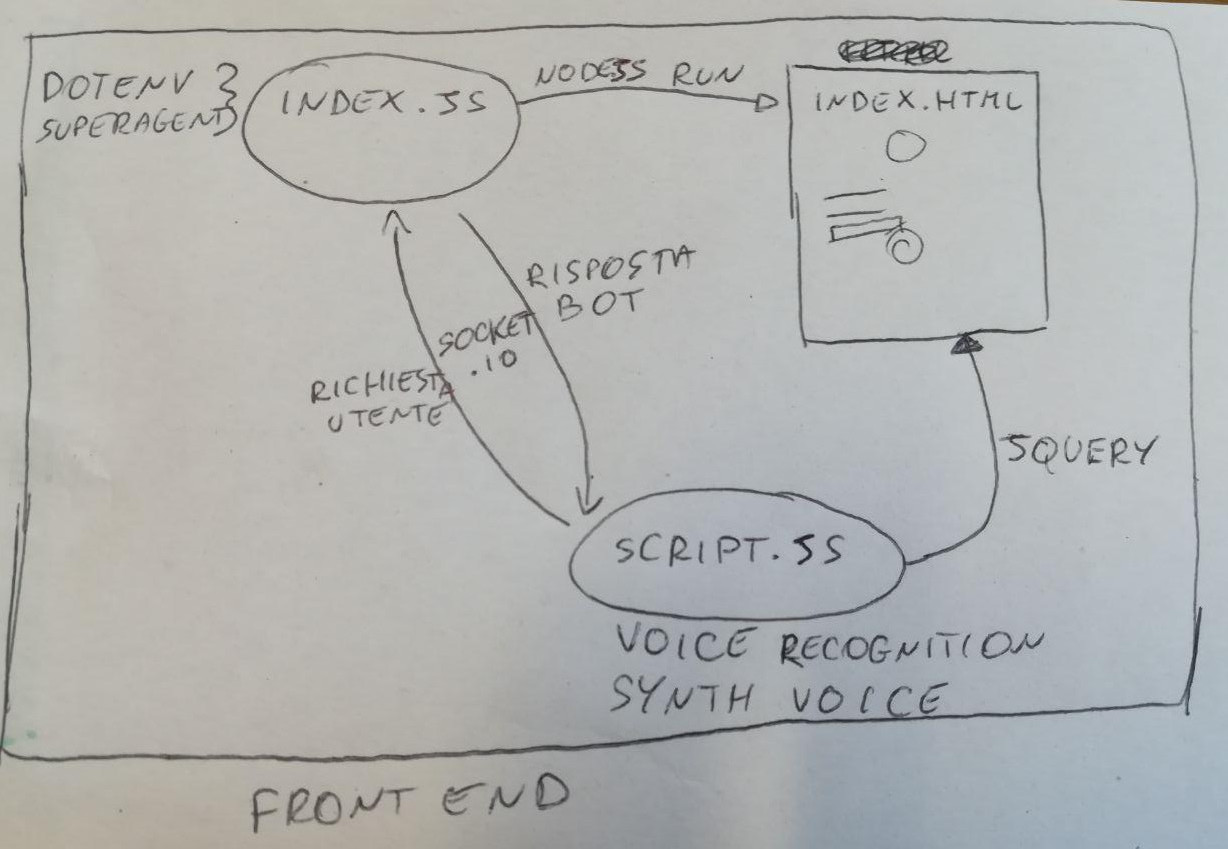
\includegraphics[width=0.8\textwidth]{img/frontend.jpg}
 \caption{Nlu data set example}
\end{figure}

\section{Creazione dell'intelligenza artificiale}
\iffalse
<inserimento della comunicazione tra la chat e dialogflow>
<vari test di funzionamento della comunicazione>
<passaggio da dialogflow a rasa>
<studio di rasa nlu>
https://en.wikipedia.org/wiki/Human_computation
https://en.wikipedia.org/wiki/AI-hard
https://en.wikipedia.org/wiki/Human_computation
https://en.wikipedia.org/wiki/Dialogflow
https://dialogflow.com/
\fi
Abbiamo trattato fino a ora la parte relativa all'utente, passiamo ora alla creazione del vero e proprio bot trasformando la chat creata in un chatbot. Quello di cui un chatbot ha bisogno \'e di analizzare la frase inviata dall'utente e generare una risposta in grado di soddisfare le richieste, sono quindi necessari 2 livelli di computazione: un'intelligenza artificiale che esegue l'analisi del testo e un'altra che in base alla storia della conversazione generi una risposta il pi\'u plausibile possibile alle richieste dell'utente.
\iffalse
Per utilizzare un sistema di risposte automatiche \'e necessario sfruttare un'intelligenza artificiale che eseguendo un'analisi della frase inviata dall'utente deve riuscire a determinare una risposta consona alla richiesta.
L'automatismo della conversazione viene gestito dal bot che per mezzo di un'architettura formata da 2 diverse intelligenze artificiali riesce a generare delle risposte e delle azioni
L'automatismo di risposta della chat viene gestito da un'intelligenza artificiale che sfruttando le metodologie del natural language understanding genera 
Per permettere la conversazione tra l'essere umano e il bot \'e necessario modellare quest'ultimo con le metodologie proprie del nlu
La funzione di risposta automatica viene gestita da un'intelligenza artificiale 
Per poter conversare il bot deve essere creato con dei sistemi di natural language understanding e un'intelligenza artificiale per eseguire azioni necessarie per comprendere e rispondere alle richieste fornite dall'utente. (dio la bruttezza dei questa frase)
\fi
\'E necessario quindi parlare di natural language understanding (NLU), una branca dell'intelligenza artificiale che cerca metodi di analisi di un testo per comprendere il significato della frase estraendo informazioni importanti. Problemi di questo tipo sono considerati AI-Hard, chiamati anche AI-Complete, cio\'e non risolvibili con un semplice algoritmo ma \'e necessaria la supervisione dell'uomo che addestra l'intelligenza a risolvere un problema specifico.
Data la complessit\'a di questo compito ho ricercato uno strumento che eseguisse la funzione di NLU e quello che mi \'e sembrato pi\'u vicino alle mie necessit\'a era lo strumento chiamato Dialogflow che forniva tutti gli strumenti necessari per quello che il bot avrebbe dovuto fare.
Dialogflow \'e un tool sviluppato da google per la creazione di conversazioni utente macchina in linguaggio naturale che permette di sfruttare una tecnologia di questo tipo in qualsiasi contesto necessario, un punto di forza di questo strumento \'e l'interfaccia web molto semplificata per utenti anche alle prime armi.
Per creare un'intelligenza artificiale di questo tipo \'e importante creare un dataset con degli esempi chiari di frasi specificando tutti gli elementi necessari, per il natural language understanding ci\'o di cui si ha bisogno \'e definire per ogni esempio: l'intento della frase e se ci sono delle entit\'a estraibili utili per creare una risposta.
L'intento \'e il concetto principale che ci permette di indicare l'obbiettivo della frase per distinguere i vari casi che possono presentarsi durante la conversazione con un utente, avere quindi un dataset con una popolazione molto varia permette avere un addestramento dell'intelligenza migliore e preciso in fase di runtime.
Le entit\'a sono invece tutti quegli oggetti che all'interno della frase risultano importanti per un uso esterno, per esempio se la richiesta dell'utente \'e il pagamento di 300 euro l'entit\'a che andremo a definire sar\'a 300 che corrisponder\'a al quantitativo di euro che dovremo richiedere di trasferire.  
Il primo dataset che ho creato con Dialogflow era formato da pochi esempi di richieste di pagamento che ho indicato con l'intento chiamato \textbf{payRequest} formato da entit\'a \textbf{receiver}, \textbf{quantity} e \textbf{currency}.
\begin{figure}[H]
 \centering
  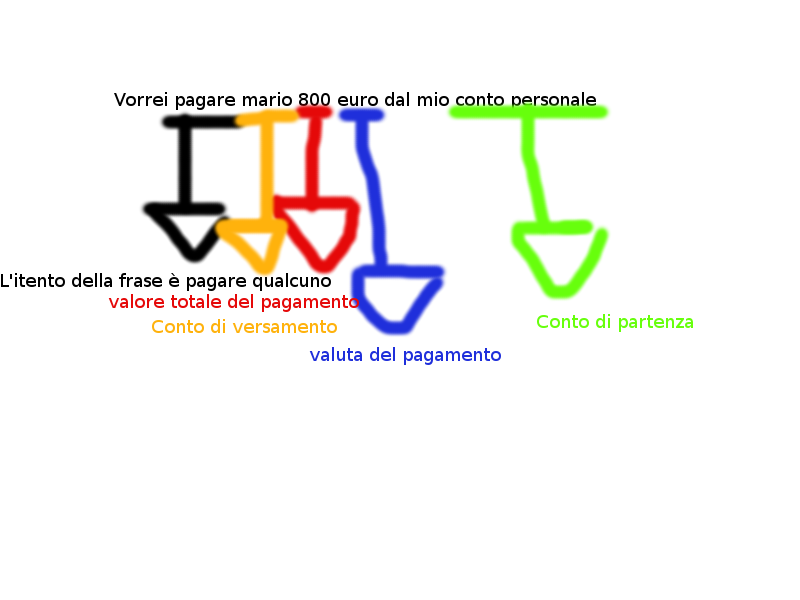
\includegraphics[width=0.8\textwidth]{img/nludatasetexample.png}
 \caption{Nlu data set example}
\end{figure}
Il motivo della creazione di un dataset ristretto mi ha permesso di integrare questo nuovo strumento con il frontend testando i metodi di conversazione e l'effettivo funzionamento della chat.
Il passo subito successivo sarebbe stato quello di sviluppare le richieste di pagamento effettive verso il gestionale della banca attraverso delle semplici chiamate get e post, in questa fase non ho ritenuto necessario preoccuparmi del problema dell'autenticazione dell'utente nel gestionale della banca rimandando il problema una volta integrato il prototipo nella web application.
Una volta presentato il prototipo funzionante sono stati creati alcuni issues riguardanti il problema della privacy dei dati degli utenti della banca. 
Il problema principale era il fatto che i dati come: iban, transazione e nome dell'utente, venivano gestiti da Dialogflow quindi da un utente terzo che avrebbe potuto usare questi dati per scopi propri, mi \'e stato di conseguenza richiesto di usare un altro strumento per eseguire queste funzioni.
Per risolvere questo problema ho cominciato a cercare progetti di tipo open source che racchiudessero tutte le funzionalit\'a fornite da Dialogflow permettendo lo sviluppo in locale e che fossero efficienti alla pari con il precendente strumento.
\iffalse
https://rasa.com/about/
https://rasa.com/docs/
\fi
Il progetto open source che ho scelto di usare \'e Rasa, framework sviluppato in Python ancora in fase di sviluppo che consente di sviluppare una intelligenza artificiale utile per chatbot di qualsiasi tipo.
Questo framework \'e diviso in 2 componenti principali: rasa\_nlu per eseguire le funzioni di natural language understanding consentendo quindi di classificare gli intenti ed estrarre le entit\'a e rasa\_core che tramite machine learning gestisce i dialoghi con l'utente. 
L'implementazione di queste due componenti nella realt\'a che dovevo relizzare comportava la creazione di un dataset molto diverso rispetto al precedente e inoltre lo sviluppo del bot era fondato sull'implementazione di una classe Python che doveva contenere le funzionalit\'a necessarie per completare le azioni richieste dal bot.
Lo sviluppo del dataset necessario a rasa\_nlu \'e formato da file di configurazione 


\section{Aggiornamento Frontend per la comunicazione con Rasa}

\section{Sistema di pagamento vocale}

\section{Funzionamento e esecuzione}

\iffalse
<creazione di un primo modello di training con vari esempi esterni al progetto>
<processo di apprendimento del funzionamento effettivo di rasa lungo>
<tentativo di utilizzo del modello creato precedentemente, con dialogflow, per la creazione del modello di rasa nlu>
<passaggio di competenze(?) da dialogflow a rasa, eliminando la comunicazione effettiva con google>
<connessione con il server bps e rasa>
<per errore ho lasciato che la chat inviasse ancora i dati di test ai server di dialogflow = rasa>dialogflow>
<tutor universitario consiglia l'uso di typescript => studio di typescript => riscrittura della chat usando typescript>
<typescript migliore lettura del codice e possibilità di creazione di classi e oggetti>
<estrapolazione dei dati utente dal server della banca usando chiamate rest>
<generazione data set dell'intelligenza artificiale>
<necessario un server che eseguisse azioni richieste>
<studiare python per poter creare esempi di rasa core>
<studio di rasa core - server>
<utilizzo di chiamate rest all'interno del chatbot verso rasa core>
<problemi con la messa in opera del server su macchina windows>
<utilizzo del server su rete locale per i test>
<refactor del codice chatbot usando superagent (vedi https://github.com/Wabri/UniversityInternship#day-26-110718--55-ore)>
<iniziato a creare le story per generare un modello efficace di intelligenza>
<Cominciato a generare le prime azioni di risposta in base agli intenti e al contenuto del testo fornito in input>
<Creato l'effettivo bot scritto in python, dove risiedono tutte le azioni che può fare il bot>
<Migliorato il modello di training aggiungendo nuovi esempi di intents e stories>
<problemi con l'autenticazione a 2 fattori per il prototipo, non riesce a estrarre direttamente user e password e devo inserirle manualmente con chiamate post verso il server rasa>
<completamento comunicazione user-rasafrontend-rasabackend-backendspringbanca - vedi https://github.com/Wabri/UniversityInternship/blob/master/README.md#day-36-020818--65-ore>
<creazione delle azioni effettive che deve fare il bot rasa backend>
<il problema del xcsrf token e jsession>
<vedi https://github.com/Wabri/UniversityInternship/blob/master/README.md#day-38-210818--75-ore per maggiori informazioni>
<documentazione prototipo>
\fi